% !TEX root = BA-Bauer.tex
\newpage
\section{Zusammenfassung}
In der vorangegangen Praxisprojektarbeit wurden Grundlagen erarbeitet, welche die Aufnahme und Wiedergabe von DMX-Datenströmen mit einem Mikrocontroller ermöglichen. Die entwickelte Hard- und Software eigneten sich nicht für eine nützliche Anwendung in der Praxis.\\
Ziel dieser Arbeit ist die Implementierung und Weiterentwicklung der erarbeiteten Grundlagen der Praxisprojektarbeit in einen Prototypen. Die Entwicklung ist auf das zukünftige Erlangen der Marktreife ausgerichtet.\\
Zum Erreichen dieses Ziels wurde eine Benutzerschnittstelle entwickelt, die eine intuitive Bedienung des Gerätes ermöglicht. Dazu gehörte die Auswahl von Hardwarekomponenten, die Entwicklung einer elektrischen Schaltung und entsprechender Software. Zudem wurde eine Platine entworfen, welche in einem passenden Gehäuse montiert wurde.\\
Das Ergebnis dieser Arbeit ist ein funktionsfähiger Prototyp mit einer deutlich erkennbaren Marktreife, zu sehen in den nachstehenden Abbildungen.
\begin{figure}[h]
	\begin{minipage}{.45\linewidth}
		\centering
		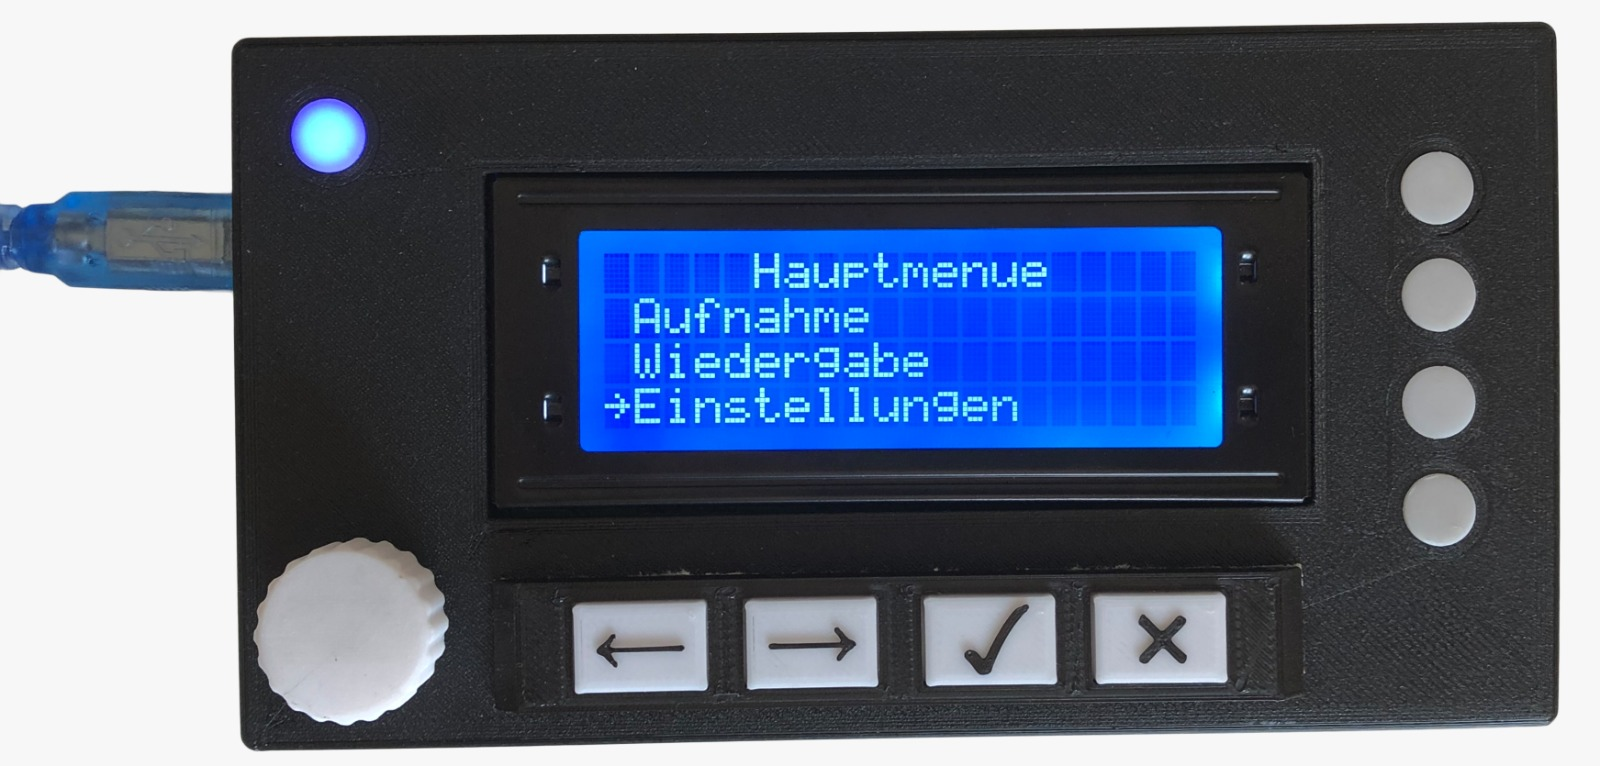
\includegraphics[height=.15\textheight]{Resultat/Vorderseite-freigestellt}
		\caption{DMX-Aufnahme- und "~Wiedergabegerät - Vorderseite}
	\end{minipage}
	\hfill
	\begin{minipage}{.45\linewidth}
		\centering
		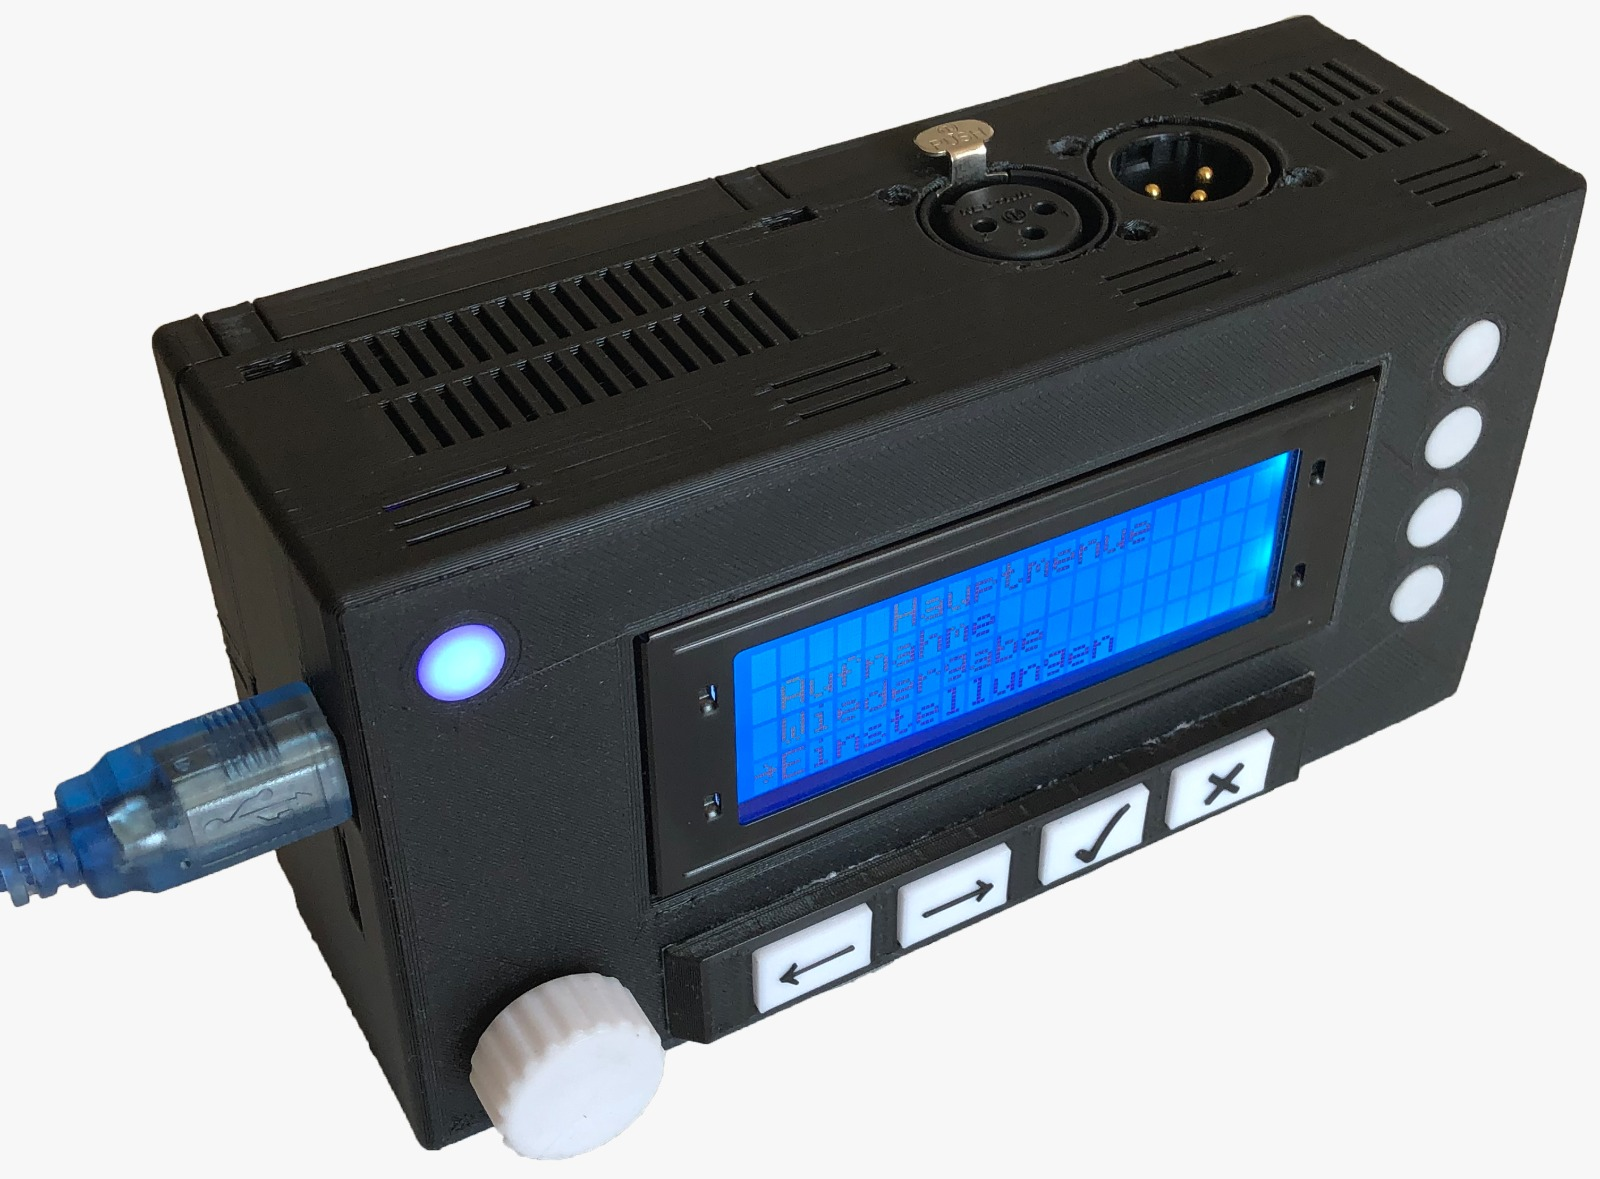
\includegraphics[height=.2\textheight]{Resultat/Aufgestellt-freigestellt}
		\caption{DMX-Aufnahme- und "~Wiedergabegerät - Rückseite}
	\end{minipage}
\end{figure}
Die Weiterentwicklung und Erweiterung der Grundlagen aus der Praxisprojektarbeit ermöglichen dem Benutzer die Aufnahme und Wiedergabe von DMX-Daten in verschiedenen Modi. Eine variabel einstellbare Aufnahmezeit und die Möglichkeit, mehrere Aufnahmen anzulegen, stellen eine deutlich praxisnähere Verwendbarkeit her. Eine Erkennung von Übertragungsfehlern während der Aufnahme lässt eine zuverlässige Aufnahme zu. Die Implementierung einer umfassenden Benutzerschnittstelle, bestehend aus einem Display, Tastern, LEDs und einem Drehgeber, ermöglicht intuitive Eingaben des Benutzers und Rückmeldungen. Nützliche Fehlermeldungen erleichtern die Behebung von eventuell auftretenden Fehlern. Statusanzeigen in Form von aufblinkenden LEDs in verschiedenen Farben lassen die Überprüfung der Funktion des Gerätes auf größere Entfernung zu. Ein Menü mit einfacher Menüführung hilft dem Benutzer alle Funktionen des Geräts intuitiv und ohne spezielle Vorkenntnisse zu verwenden. Über die Einstellungsmöglichkeiten kann der Benutzer die Funktion des Gerätes und die Optik der Benutzerschnittstelle auf die persönlichen Bedürfnisse anpassen. Ein Gehäuse in einer handlichen Größe lässt eine Vielzahl an Einsatzgebieten zu.\\
Die in der Praxisprojektarbeit erarbeiteten Grundlagen sind erfolgreich in einen Prototypen implementiert. Dieser bietet das Potential einer Weiterentwicklung bis zum Erlangen der tatsächlichen Marktreife. An der Hardware sind dafür wenige Änderungen vorzunehmen. Die Konstruktion des Gehäuses sollte für die Herstellung mit einem Spritzgussverfahren ausgelegt werden um eine Serienproduktion zu vereinfachen. Gleichzeitig müssen die Zugänglichkeit der SD-Karte und der Taster-Mechanismus optimiert werden. Der ungenutzte Raum im Gehäuse, könnte mit einem Akku für mobile Anwendungen belegt werden. Auch die Software muss für die Marktreife optimiert werden. Einige spezielle Fälle, in denen Einstellungen getroffen werden können, die technisch nicht umsetzbar sind, werden nicht abgefangen. So ist es derzeit möglich, eine Aufnahmezeit zu wählen, die technisch nicht erreicht werden kann. Auch die Benutzerschnittstelle kann an einigen Stellen optimiert werden, um unbeabsichtigte Eingaben des Benutzers zu filtern. Eine Erweiterung der maximal 20 möglichen Aufnahme-Dateien ist außerdem sinnvoll. Der Speicherbedarf könnte optimiert werden und eine Fehlerkorrektur und eine genauere Fehlererkennung könnten Datenverlust verringern.
%Software
%		max 20 Aufnahmen
%		Interbytedelay
%		Optimierung Speicherbedarf / Fehlererkennung und -korrektur
% 		Optimierung GUI
% 		Tastertimeout
%Hardware
%		Tasterflächen
%		Zugänglichkeit SD-Karte